\documentclass{article}
\usepackage{tikz}
\usepackage{float}
\usepackage{enumerate}
\usepackage{amsmath}
\usepackage{bm}
\usepackage{indentfirst}
\usepackage{siunitx}
\usepackage[utf8]{inputenc}
\usepackage{graphicx}
\graphicspath{ {Images/} }
\usepackage{float}
\usepackage{mhchem}
\usepackage{chemfig}
\allowdisplaybreaks

\title{ 8.01 Problem Set 11 }
\author{ Robert Durfee - Lecture 7 - Table 9 }
\date{ November 27, 2017 }

\begin{document}

\maketitle

\section{ Cubical Block Collision with Low Ridge }

\subsection*{ Part A }

Since the axis of rotation is not around the center of mass, the moment of
interia about the edge of the cube must be computed using the paralell axis
theorem.
\begin{align*}
    I &= I_{cm} + md^{2} \\
    I &= \frac{1}{6} ms^{2} + \frac{1}{\sqrt{ 2 }} ms^{2} \\
    I &= \frac{2}{3} ms^{2}
\end{align*}

Using an axis along the horizontal surface, angular momentum is conserved:
\begin{align*}
    \frac{1}{2} mvs &= \frac{2}{3} ms^{2}\omega \\
    \omega &= \frac{3v}{4s}
\end{align*}

\subsection*{ Part B }

After the collision, the mechanical energy of the block is conserved. Thus,
using the angular speed calculated in Part B:
\begin{align*}
    \frac{1}{2} I\omega^{2} + mgh_{cm,0} &= mgh_{cm,f} \\
    \frac{3}{16} msv^{2} + \frac{1}{2} mgs &= \frac{1}{\sqrt{ 2 }} mgs \\
    v &= 2 \sqrt{ \frac{2gs}{3} \left( \sqrt{ 2 } - 1 \right) }
\end{align*}

\section{ Yo-Yo Rolling on Inclined Plane }

Before the yo-yo starts slipping, we can assume that it rolls clockwise, in the
direction of the applied force. As a result, positive angular acceleration is
clockwise and positive linear acceleration is up the plane. Thus, the force and
torque equations are as follows:
$$ R\mu_{s}mg \cos \left( \phi \right) - \frac{ R }{ 3 }F = \frac{ 1 }{ 2 } mRa $$
$$ F - mg \sin \left( \phi \right) - \mu_{s}mg \cos \left( \phi \right) = ma $$

Solving this system of equations for $F$ results in:
$$ \frac{ 3 }{ 5 } \left( 3 \mu_{s} \cos \left( \phi \right) - \sin \left( \phi
\right) \right) = F$$

\section{ Billiards }

\subsection*{ Part A }

During the collision between the billiard ball and the cue stick, since friction
can be ignored (as stated in the problem), the only force acting on the billiard
ball is the impulse by the cue stick. As a result, the angular momentum of the
billiard ball, if the axis is taken to be along the direction the impulse is
applied, is conserved. Also, since the billiard is initially at rest, this
angular momentum sums to zero.

After the collision between the billiard call and the cue stick, friction cannot
be ignored, but it is the only force acting on the billiard ball. Thus, angular
momentum of the billiard ball is conserved about the axis along the direction of
friction. Initial and final angular momentum of the billiard ball can be
calculated from this.

\subsection*{ Part B }

Initial and final angular momentum before and after the cue stick hits the
billiard ball are:
$$ L_{i} = 0 $$
$$ L_{f} = mv_{0}h - I\omega_{0} $$

Setting these two equal, as angular momentum is conserved about the chosen axis,
yields:
\begin{equation} 
    mv_{0}h = I\omega_{0} 
\end{equation}

Now, after the collision as the billiard ball begins to accelerate due to the
frictional force, the initial and final angular momentum can be written about an
axis along the surface:
\begin{equation} 
    L_{i} = mv_{0}R + I\omega_{0} 
\end{equation}
\begin{equation} 
    L_{f} = mv_{f}R + I\omega_{f} 
\end{equation}

Using our result from equation 1 and plugging it into equation 2 results in:
\begin{equation}
    L_{i} = mv_{0}( R + h )
\end{equation}

Using our result from equation 3 and the supplied values of $v_{f}$ and $I$: 
\begin{equation}
    L_{f} = \frac{ 9mv_{0}R }{ 5 }
\end{equation}

Equating equations 4 and 5 results in:
$$ \frac{ h }{ R } = \frac{ 4 }{ 5 } $$

\section{ Grain Mill }

\subsection*{ Part A }

Given that the wheel rotates without slipping,
$$ \omega b = v $$

Where $v$ is the instantaneous tangental velocity around the pivot, $P$. Thus,
$$ \frac{ \omega b }{ R } = \Omega $$

Rearranging this to solve for $\omega$:
$$ \omega = \frac{ \Omega R }{ b } $$

\subsection*{ Part B }

The angular momentum of the wheel around the pivot, $P$:
$$ L = I\omega $$

Substituting for the moment of interia and the value computed for $\omega$:
$$ L = \frac{ Mb\Omega R }{ 2 } $$

Using the right hand rule, the direction of angular momentum can be found:
$$ \vec{ L } = -\frac{ Mb\Omega R }{ 2 } \hat{ r } $$

\subsection*{ Part C }

\begin{figure}[H]
    \centering
    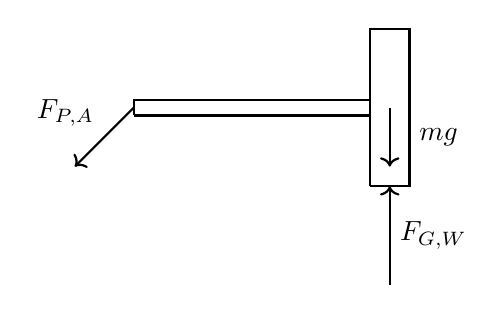
\begin{tikzpicture}
        \draw [ thick ] ( 0,-0.10 ) -- ( 0,0.1 ) -- ( 3,0.1 );
        \draw [ thick ] ( 0,-0.10 ) -- ( 3,-0.10 );
        \draw [ thick ] ( 3,-1 ) -- ( 3,1 ) -- ( 3.5,1 ) -- ( 3.5,-1 ) -- ( 3,-1
        );
        \draw [ thick, -> ] ( 0,0 ) -- ( -0.75,-0.75 ) node[ anchor = south east,
        pos = 0.5]{ $F_{P,A}$ };
        \draw [ thick, -> ] ( 3.25, 0 ) -- ( 3.25, -0.75 ) node[ anchor = west,
        pos = 0.5, xshift = 7 ]{ $mg$ };
        \draw [ thick, -> ] ( 3.25, -2.25 ) -- ( 3.25, -1 ) node[ anchor = west,
        pos = 0.5 ]{ $F_{G,W}$ };
    \end{tikzpicture}
\end{figure}

\subsection*{ Part D }

Only the normal force from the ground onto the wheel and the weight force from
the wheel contribute to the torque about the pivot. Since we know that the
normal force is twice the weight of the wheel, the torque can be written:
$$ \tau = -2MgR + MgR = -MgR $$

Using the right hand rule, a direction can be ascribed:
$$ \vec{ \tau } = -MgR \hat{ \theta } $$

\subsection*{ Part E }

Using the relationship between torque and change in angular momentum:
$$ \tau = \frac{ dL }{ dt } $$

And the relation derived in class of change in angular momenutm and processional
angular speed:
$$ \frac{ dL }{ dt } = \vert L \vert \Omega $$

Combining the torque and angular momentum as computed above:
$$ \Omega = \sqrt{ \frac{ 2g }{ b } } $$

\section{ Gyroscope on Rotating Platform }

\subsection*{ Part A }

Each force exerts a torque on the center of mass a distance $d$ away, but they
both point in opposite directions.
$$ \tau = d( F_{a} - F_{b} ) $$

Using the right hand rule, the direction of torque is in the $\theta$ direction:
$$ \vec{ \tau } = d( F_{a} - F_{b} ) \hat{ \theta } $$

\subsection*{ Part B }

Newton's second law states:
$$ \tau = \frac{ dL }{ dt } $$

We derived a relation between $L$ and $\Omega$:
$$ \frac{ dL }{ dt } = \vert L \vert \Omega $$

Substituting our value for torque and angular momentum:
$$ F_{a} - F_{b} = \frac{ I \omega \Omega }{ d } $$

\subsection*{ Part C }

The force version of Newton's second law:
$$ F_{a} + F_{b} - Mg = 0 $$

Solving for $F_{a}$:
$$ F_{a} = \frac{ 1 }{ 2 } \left( Mg + \frac{ I \omega \Omega }{ d } \right) $$

Solving for $F_{b}$:
$$ F_{b} = \frac{ 1 }{ 2 } \left( Mg - \frac{ I \omega \Omega }{ d } \right) $$

\section{ Upward Tiled Gyroscope }

\subsection*{ Part A }

The only force that produces a torque is the weight of the gyroscope, which is
pointing in an angle $\phi$, with respect to the axis:
$$ \tau = mgl \cos( \phi ) $$

Using the right hand rule, applying direction:
$$ \vec{ \tau } = mgl \cos( \phi ) \hat{ \theta } $$

\subsection*{ Part B }

Newton's second law states:
$$ \tau = \frac{ dL }{ dt } $$

We derived a relation between $L$ and $\Omega$:
$$ \frac{ dL }{ dt } = \vert L \vert \Omega $$

Substituting our values for torque and angular momentum:
$$ \Omega = \frac{ mgl }{ I \omega_{s} } $$

Note: the $\cos( \phi )$ cancels out because we use the horizontal component of
angular momentum above.

Since this value is positive, the procession is clockwise.

\subsection*{ Part C }



\end{document}

